% This work is licensed under the Creative Commons
% Attribution-NonCommercial-ShareAlike 4.0 International License. To view a copy
% of this license, visit http://creativecommons.org/licenses/by-nc-sa/4.0/ or
% send a letter to Creative Commons, PO Box 1866, Mountain View, CA 94042, USA.

\chapter{Martingalkonvergenz und gleichgradige Integrierbarkeit} %4
%\setcounter{section}{4} %kleiner Hack

\section{Martingalkonvergenz}
\underline{Vorüberlegung:} Sei $(a_n)_{n\in\N}\subseteq\R$ deterministische Folge in $\R$.
\begin{itemize}
\item $\liminf\limits_{n\to\infty} a_n$ und $\limsup\limits_{n\to\infty} a_n$ immer wohldefiniert mit Werten in $\overline{\R}:=\R\cup\lbrace\pm\infty\rbrace$
\item Grenzwert $\limn a_n$ existiert in $\overline{\R}$
\begin{align*}
\Longleftrightarrow\liminf\limits_{n\to\infty} a_n=\limsup\limits_{n\to\infty} a_n
\end{align*}
\item Mit Kontraposition gilt also 
\begin{align*}
&\lim a_n\text{ existiert \ul{nicht} in }\overline{\R}\\
&\Longleftrightarrow\liminf\limits_{n\to\infty} a_n<\limsup\limits_{n\to\infty} a_n\\
&\Longleftrightarrow
\exists p,q\in\Q\mit p<q:\liminf\limits_{n\to\infty} a_n<p<q<\limsup\limits_{n\to\infty} a_n\\
&\Longleftrightarrow
\exists p,q\in\Q\mit p<q:\\
&\qquad(a_n)_{n\in\N}\text{ unendlich oft den Streifen }[p,q]\times\N\text{ ``aufsteigend'' überquert}\\
&\Longleftrightarrow
\exists p,q\in\Q\mit p<q:U[p,q]=\infty
\end{align*}
wobei $U[p,q]$ die \textbf{upcrossings} (aufsteigende Überquerungen) des Streifens $[p,q]\times\N$ bezeichnet.
\end{itemize}

\begin{figure}[h!]
	\begin{center}
		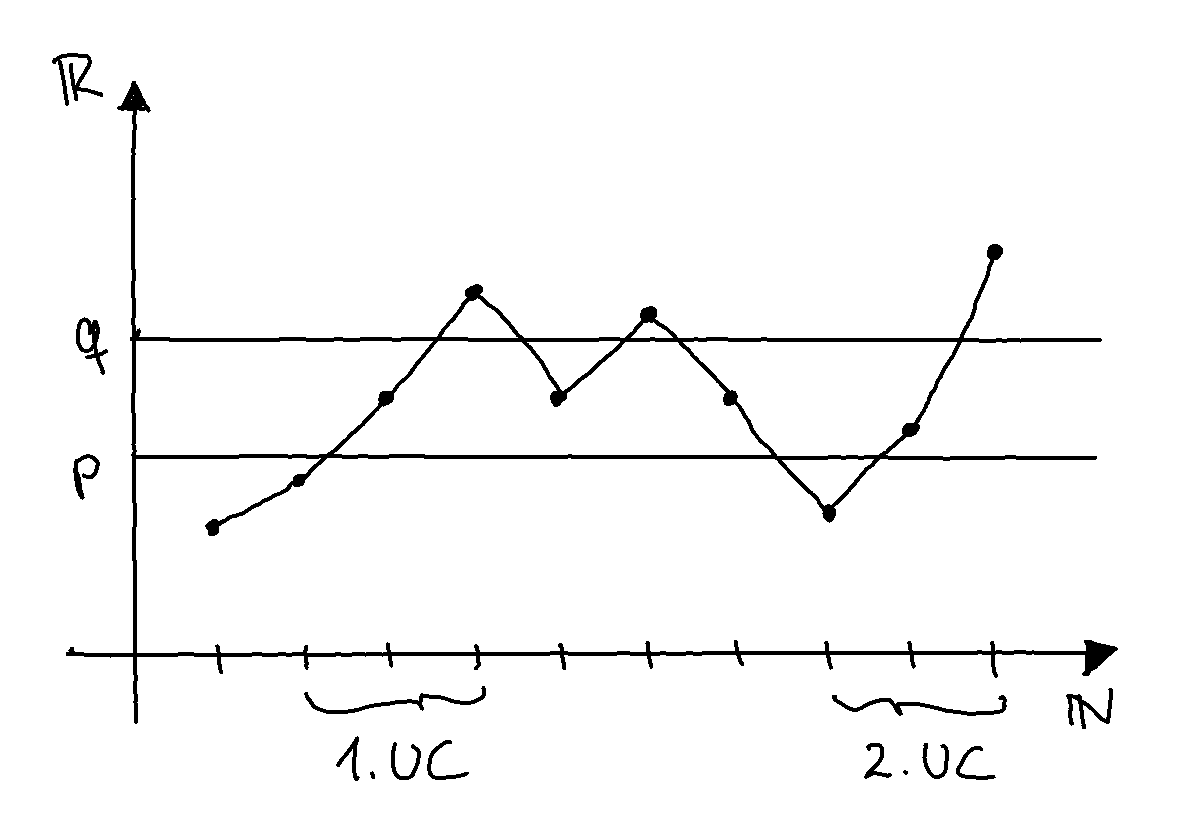
\includegraphics[width=0.75\textwidth]{./pics/Sketch2.png}
		\caption{Beispiel für Upcrossings}
		\label{AbbUpcrossing}
	\end{center}
\end{figure}

\begin{defi}
Sei $(X_n)_{n\in\N}$ ein adaptierter stochastischer Prozess und $p,q\in\R$ , $p<q$ , $N\in\N$. Setze % Die einzelnen $..$ Umgebungen sind hier wichtig, sonst passiert ein Zeilenumbruch inmitten der Matheumgebung
\begin{align*}
	U_N[p,q]:=\max\left\{ k\in\N_0\left|
\begin{array}{c}
	\exists\text{ Stoppzeiten }0<\sigma_1<\tau_1<\sigma_2<\tau_2<\ldots<\tau_k\le N\\
	\forall i\in\lbrace 1,\ldots,k\rbrace: X_{\sigma_i}<p \text{ und } X_{\tau_i}>q
\end{array}\right.\right\} % hier Wort "und" da sonst Verwirrung mit minimum
\end{align*}
$U_N[p,q]$ ist die Anzahl der \textbf{Upcrossings} von $[p,q]\times\lbrace0,1,\ldots,N\rbrace$ durch $(X_n)_{n\in\N}$ und 
\begin{align*}
U[p,q]=\limsup\limits_{n\to\infty} U_n[p,q]
\end{align*}
die Anzahl der \textbf{Upcrossings} von $[p,q]\times\N$.
\end{defi}

\setcounter{section}{4} %fix numbering
\begin{lemma}[Doob's Upcrossing Lemma]\enter\label{lemma4.1DoobsUpcrossingLemma}
Sei $(X_n)_{n\in\N}$ Sub-Martingal und $p,q\in\R\mit p<q$. Dann gilt:
\begin{align*}
\E\big[U_N[p,q]\big]&\leq\frac{\E\big[(X_N-p)^+\big]}{q-p}\qquad\forall N\in\N
\end{align*}
\end{lemma}

\begin{bemerkung}
\textbf{Positivteil} und \textbf{Negativteil} einer Zufallsvariblen $X$ ist definiert als
\begin{align*}
X^+(\omega):=\max\big\lbrace X(\omega),0\big\rbrace
\qquad\text{ und }\qquad
X^-(\omega):=-\min\big\lbrace X(\omega),0\big\rbrace
\end{align*}
Es gilt $X=X^+-X^-$ und $|X|=X^++X^-$.
\end{bemerkung}

\begin{proof}
Setze der Kürze halber $k(\omega):=U_N[p,q](\omega)$. Klarerweise ist $k\leq N$. Definiere
\begin{align*}
\tau_0&:=0\\
\sigma_j&:=\min\big\lbrace k\geq \tau_{j-1}:X_k<p\big\rbrace\wedge N\text{ ``Erstaustrittszeit''}\\
\tau_j&:=\max\big\lbrace k\geq\sigma_j:X_k>q\big\rbrace\wedge N
\end{align*}
d. h. $\tau_0<\overbrace{\sigma_1<\tau_1}^{\text{1. Upcrossing}}<\overbrace{\sigma_2<\ldots}^{\text{2. Upcrossing}}\ldots<\tau_k$ und $\tau_{k+1}=\sigma_{k+1}=\tau_{k+2}=\ldots=\tau_N=N$. Es gilt:
\begin{align}\label{eqProof4.1.1Stern}\tag{$\ast$}
(q-p)\cdot U_N[p,q] &\leq
\overbrace{\underbrace{(X_{\tau_1}-p)}_{>q-p}+\underbrace{(X_{\tau_2}-X_{\sigma_2})}_{>q-p}+\ldots+\underbrace{(X_{\tau_k}-X_{\sigma_k})}_{>q-p}}^{U_N[p,q]\text{ Summanden}}
\end{align}
Außerdem gilt
\begin{align}\label{eqProof4.1.1ZweiStern}\tag{$\ast\ast$}
\min\lbrace X_N-p,0\rbrace&\leq X_N-X_{\sigma_{k+1}},
\end{align}
denn: 
\begin{align*}
X_N-p<0&\implies X_{\sigma_{k+1}}<p&\implies X_N-p\leq X_{\sigma_{k+1}}-p\\
X_N-p\geq0&\implies \sigma_{k+1}=N&\implies X_N-p- X_{\sigma_{k+1}}=0
\end{align*}
Addiere von \eqref{eqProof4.1.1Stern} auf \eqref{eqProof4.1.1ZweiStern}
\begin{align*}
	(q-p)\cdot U_N[p,q]+\underbrace{\min\lbrace X_N-p,0\rbrace}_{\stackeq{\text{def}}-(X_N-p)^-}\leq (X_{\tau_1}-p) + \sum_{i=2}^N (X_{\tau_i} - X_{\sigma_i})
\end{align*}
Bilden von Erwartungswert und Umordnen der Summe liefert
\begin{align*}
(q-p)\cdot\E\big[U_N[p,q]\big]-\E\big[(X_N-p)^-\big]
&\leq\E[X_N]-\left(p+\sum\limits_{j=1}^{N-1}\Big(\underbrace{\E\big[X_{\sigma_{j+1}}\big]-\E\big[X_{\tau_j}\big]}_{\geq 0\text{, wegen Theorem \ref{theorem3.4}}}\Big)\right)\\
&\leq\E\big[(X_N-p)\big]\\
\implies
(q-p)\cdot\E\big[U_N[p,q]\big]&\leq\E\big[(X_N-p)+(X_N-p)^-\big]\\
&=\E\big[(X_N-p)^+\big]
\end{align*}
\end{proof}

\begin{theorem}[Martingalkonvergenz]\label{theorem4.2Martingalkonvergenz}\enter
Sei $(X_n)_{n\in\N}$ ein Submartingal mit $\sup\limits_{n\in\N}\E[X_n^+]<\infty$. Dann gilt:
\begin{align*}
\exists X_\infty\in L_1(\Omega,\A,\P):\limn X_n=X_\infty\text{ fast sicher}
\end{align*}
\end{theorem}
\begin{proof}
Zunächst zeigen wir den Satz für $X_\infty$ mit Werten in $\overline{\R}$. Mit Vorüberlegung (zu Beginn des Kapitels) reicht es zu zeigen:
\begin{align*}
\P\big(U[p,q]=\infty\big)=0\qquad\forall p,q\in\Q\mit p<q
\end{align*}
denn:
\begin{align*}
\P\left(\limn X_n\text{ exisitiert nicht in }\overline{\R}\right)
&=\P\left(\bigcup\limits_{\begin{subarray}{c}p,q\in\Q\\ p<q\end{subarray}}\big\lbrace U[p,q]=\infty\big\rbrace\right)\\
&\leq\sum\limits_{p,q\in\Q}\P\big(U[p,q]=\infty\big)\\
&=0
\end{align*}
Mit Lemma \ref{lemma4.1DoobsUpcrossingLemma} gilt:
\begin{align*}
\E\big[U[p,q]\big]&\stackeq{\text{Mono}}\limsup\limits_{N\to\infty}\E\big[U_N[p,q]\big]\\
&\stackrel{\ref{lemma4.1DoobsUpcrossingLemma}}{\leq}
\limsup\limits_{N\to\infty}\frac{\E\big[(X_N-p)^+\big]}{q-p}\\
&\leq\limsup\limits_{N\to\infty}\frac{\E[X_N^+]+p}{q-p}\\
&\stackrel{\text{Vor}}{<}
\infty\qquad\forall p,q\in\Q\mit p<q\\
\implies
\P\big(U[p,q]<\infty\big)&=1
\end{align*}
Also existiert $X_\infty$ mit Werten in $\overline{\R}$ und $\limn X_n=X_\infty$ fast sicher.\\
Noch zu zeigen: $X_\infty\in(-\infty,\infty)$ fast sicher und $\E\big[|X_\infty|\big]<\infty$.\\
Mit $|X|=2\cdot X^+-X$ gilt
\begin{align*}
\E\left[\limn|X_n|\right]
&\stackrel{\text{Fatou}}{\leq}
\liminf\limits_{n\to\infty}\E\big[|X_n|\big]\\
&=\liminf\limits_{n\to\infty}\Big(2\cdot\E[X_n^+]-\underbrace{\E[X_n]}_{\stackrel{\text{SubM}}{\geq}\E[X_0]}\Big)\\
&\leq
2\cdot\underbrace{\sup\limits_{n\in\N}\E[X_n^+]}_{\stackrel{\text{Vor}}{<}\infty}-\E[X_0]\\
&<\infty\\
\implies\E\big[|X_\infty|\big]&<\infty
\end{align*}
Insbesondere gilt $X_\infty\in(-\infty,\infty)$.
\end{proof}

\begin{bemerkung}
Aus Theorem \ref{theorem4.2Martingalkonvergenz} folgt \ul{nicht} die stärkere $L_1$-Konvergenz\\ $\E\big[|X_n-X_\infty|\big]\longrightarrow0$.\\
Gegenbeispiel: siehe Übungsblatt 2, Aufgabe 3
\begin{align*}
M_n^u:=\exp\left(u\cdot X_n-\frac{n\cdot\sigma^2\cdot u^2}{2}\right)\mit X_n=\xi_1+\ldots+\xi_n\text{ Random-Walk},\xi\sim\mathcal{N}(0,\sigma^2)
\end{align*}
In der Übung wurde gezeigt:
\begin{align*}
\limn M_n=0\text{ fast sicher}\qquad\forall u\neq0
\end{align*}
aber
\begin{align*}
\E\big[|M_n^u-0|\big]=\E[M_n^u]=1 \text{ keine $L_1$-Konvergenz!}
\end{align*}
\end{bemerkung}

\begin{beisp}[Wählermodell]\enter
Wähle $L,d\in\N$. Betrachte $L^d$ Individuen auf dem regelmäßigen Gitter\\ $\Lambda:=\lbrace 0,1,\ldots,L-1\rbrace^d$
\begin{figure}[h!]
	\begin{center}
		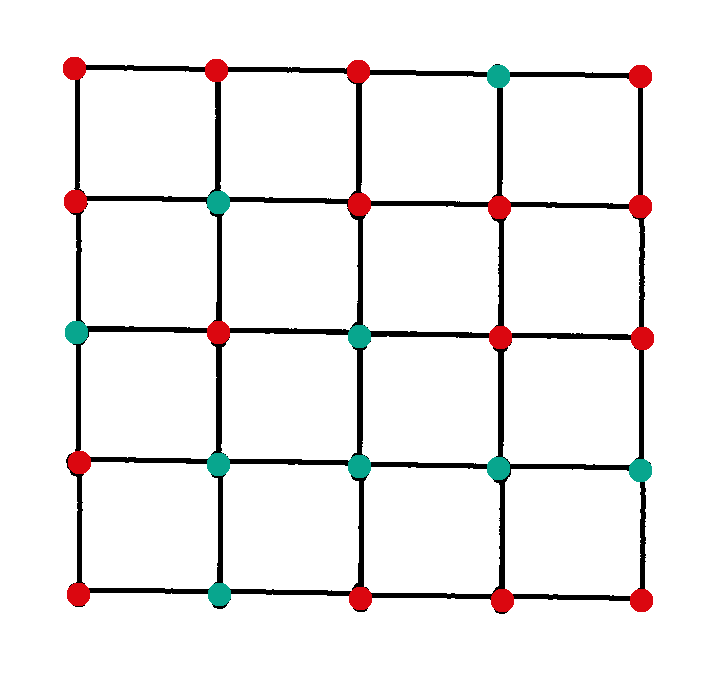
\includegraphics[width=0.5\textwidth]{./pics/Sketch1.png}
		\caption{Individuen-Gitter für $d=2$ und $L=4$}
		\label{AbbGitter}
	\end{center}
\end{figure}

Jedes Individuum hat Meinung in $\lbrace0,1\rbrace$, also dafür oder dagegen. Zustand des Kollektivs:
$x\in\lbrace0,1\rbrace^{\Lambda}=\big\lbrace f:\Lambda\to\lbrace 0,1\rbrace\big\rbrace=\lbrace0,1\rbrace^{L^d}$\\

\ul{Meinungsbildungsprozess:} Zu jedem Zeitpunkt $n\in\N_0$ übernimmt ein (zufällig ausgewähltes) Individuum $I_n$ die Meinung eines (zufällig ausgewählten) Nachbarn $I_n+N_n$. (Konvention: Es gibt keinen Rand, es wird modulo $L$ gerechnet.)\\

\ul{Mathematische Formulierung}: $(I_n,N_n)_{n\in\N_0}$ iid mit 
\begin{itemize}
\item $I_n$ $\ldots$ gleichverteilt auf dem Gitter $\Lambda$
\item $N_n$ $\ldots$ gleichverteilt auf $(\pm e_i)_{i\in\lbrace1,\ldots,d\rbrace}$
\end{itemize}
\ul{Meinungsprozess:} $X_n$ ist eine Folge von Zufallsvariablen mit Werten in Zustandsraum $\lbrace0,1\rbrace^\Lambda$ mit
\begin{align*}
X_n(i)=\left\lbrace\begin{array}{cl}
X_{n-1}(i), &\falls i\neq I_n\\
X_{n-1}(i+N_n),&\falls i=I_n
\end{array}\right.\qquad\forall i\in\Lambda
\end{align*}
\ul{Fragen:}
\begin{itemize}
	\item Langzeitverhalten?
	\item Tritt Konsens ein?
\end{itemize}
Definiere das Martingal $M_n:=$ ``Anzahl der Individuen mit Meinung 1``, also
\begin{align*}
M_n:=\sum\limits_{i\in\Lambda} X_n(i),\qquad \F_n:=\sigma\Big((I_k,N_k))_{k\in\lbrace1,\ldots,n\rbrace}\Big)
\end{align*}
\ul{Behauptung:} $M_n$ ist Martingal.
\begin{itemize}
\item Adaptiertheit: Klar nach Definition von $\F_n$
\item Integrierbarkeit: $M_n$ ist sogar beschränkt: $0\leq M_n\leq L^d$
\item Martingal-Eigenschaft:
\begin{align*}
M_n-M_{n-1}
&=\underbrace{X_{n-1}(I_n+N_n)}_{\text{vom Nachbarn übernommen}}-\underbrace{X_{n-1}(I_n)}_{\text{alte Meinung}}\\
\implies&\E\big[M_n-M_{n-1}~\big|~\F_{n-1}\big]\\
&=\E\big[X_{n-1}(I_n+N_n)-X_{n-1}(I_n)~\big|~\F_{n-1}\big]\\
&=\sum\limits_{i\in\Lambda} X_{n-1}(i)\cdot\P\big(i=\underbrace{I_n+N_n)~\big|~\F_{n-1}}_{\unab}\big)-X_{n-1}(i)\cdot\P\big(\underbrace{i=I_n~\big|~\F_{n-1}}_{\unab}\big)\\
&=\sum\limits_{i\in\Lambda} X_{n-1}(i)\cdot\Big(\underbrace{\P(i=I_n+N_n)}_{=L^{-d}}-\underbrace{\P(I_n=i)}_{=L^{-d}}\Big)\\
&=0
\end{align*}
\end{itemize}
Folglich ist $(M_n)$ ein beschränktes Martingal und somit existiert gemäß Theorem \ref{theorem4.2Martingalkonvergenz} $M_\infty\mit\limn M_n=M_\infty$ (Achtung extra Annahme: und in $L_1\implies\E[M_\infty]=\E[M_0]$).\\

\ul{Weitere Behauptung:} $M_\infty\in\lbrace 0,L^d\rbrace$, d.h. im Grenzwert gibt es nur extreme Zustände (Konsens).\\

\ul{Vorüberlegung:} Sei $x\in\lbrace0,1\rbrace^{\Lambda}$ \ul{kein} extremer Zustand, d. h. es existieren Nachbarn $i,j$ mit $X_n(i)\neq X_n(j)$.
\begin{align}
\P(X_n\neq X_{n-1}~|~X_{n-1}=x)\nonumber
&\geq \P\big(I_n=i~\&~ I_n+N_n=j~(\text{mod } L)\big)\\
&=\P\big(\underbrace{I_n=i~\&~ N_n=i-j}_{\unab}~(\text{mod  }L)\big)\nonumber\\
&=\P\big(I_n=i\big)\cdot\P\big(N_n=i-j~(\text{mod  }L)\big)\nonumber\\
&=L^{-d}\cdot\frac{1}{2\cdot d}\label{eqExampleWaehlermodellStern}\tag{$\ast$}
\end{align}
Der Kompensator $\langle M\rangle_n$ erfüllt
\begin{align*}
(M_n-M_0)^2-\langle M\rangle_n\text{ ist Martingal}\\
\implies
\E\big[\langle M\rangle_n\big]=\E\left[(M_n-M_0)^2\right]
\end{align*}
Andererseits gilt:
\begin{align*}
\langle M\rangle_n 
&=\sum\limits_{k=1}^n\E\left[\left.\underbrace{(M_k-M_{k-1})^2}_{\in\lbrace0,1\rbrace}~\right|~\F_{k-1}\right]\\
&=\sum\limits_{k=1}^n0 \cdot \P\big(X_k= X_{k-1}~\big|~\F_{k-1}\big)+ 1 \cdot \P\big(X_k\neq X_{k-1}~\big|~\F_{k-1}\big)\\
\implies
\E\big[\langle M\rangle_n\big]
&\stackeq{\text{tower}}\sum\limits_{k=1}^n\P\big(X_k\neq X_{k-1}\big)\\
&=\sum\limits_{k=1}^n\underbrace{\P\big(X_k\neq X_{k-1}~|~ M_{k-1} \in \{0,L^d\}\big)}_{\geq 0} + \P\big(\underbrace{X_k\neq X_{k-1}~|~ M_{k-1} \not\in \{0,L^d\}}_{\unab}\big)\\
&\stackrel{\eqref{eqExampleWaehlermodellStern}}{\geq}
\sum\limits_{k=1}^n L^{-d}\cdot\frac{1}{2\cdot d}\cdot\P\big(\underbrace{M_{k-1}\not\in\lbrace0,L^d\rbrace}_{=:A_{k-1}\text{ (kein extremer Zustand)}}\Big)
\end{align*}
Außerdem:

\begin{align*}
L^{2\cdot d}
&\geq \E\left[(M_n-M_0)^2\right]\\
&=\E\big[\langle M\rangle_n\big]\\
&\geq L^{-d}\cdot\frac{1}{2\cdot d}\cdot\sum\limits_{k=1}^n\P(A_{k-1})\\
\implies
\sum\limits_{k=1}^n\P(A_{k-1})&\leq L^{3\cdot d}\cdot 2\cdot d<\infty
\end{align*}

Satz von Borel-Cantelli: Nur endlich viele Ereignisse $(A_k)_{k\in\N}$ treten ein, d.h.
\begin{align*}
&\exists N_0:\Omega\to\N:\forall n\geq N_0(\omega):\omega\not\in A_n\\
&\implies M_n(\omega)\in\lbrace0,L^d\rbrace\qquad\forall N_0(\omega)\\
&\implies M_\infty:=\limn M_n\text{ nimmt nur extreme Werte $\lbrace0,\Lambda^d\rbrace$ an!}
\end{align*}
Im Grenzwert tritt perfekter Konsens auf!
\begin{align*}
\P\big(M_\infty=L^d\big)&=L^{-d}\cdot\E[M_\infty]\stackeq{L_1\text{-Konv}} L^{-d}\cdot\E[M_0]\\
\P(M_\infty=0)&=1-L^{-d}\cdot\E[M_0]
\end{align*}
\end{beisp}




%Abschließbar: $X_n=\E[X_\infty~|~\F_n]$?


